%!\subsection{Quantitative complexity Analysis}
%    \label{subsec:ComplexityImageAnalysis}
%    %!\subsection{Quantitative complexity Analysis}
%    \label{subsec:ComplexityImageAnalysis}
%    %!\subsection{Quantitative complexity Analysis}
%    \label{subsec:ComplexityImageAnalysis}
%    %!\subsection{Quantitative complexity Analysis}
%    \label{subsec:ComplexityImageAnalysis}
%    \input{Text/ResultsImageComplexityAnalysisHistory.tex}

We have previously discussed the argument that the architectural evolution, throughout history, has been characterized by a continual interplay between simplicity and complexity.
This notion has been substantiated by our exploration of the theoretical definitions and varied approaches to facades and ornamentation within the context of prominent architectural styles and the perspectives of their eminent architects.

Our literature review has consistently pointed towards a prevailing trend in contemporary architecture, suggesting a resurgence of complexity in architectural design.
However, to ensure our findings are not purely subjective or biased towards this conclusion, we have conducted a quantitative analysis using the Computational Image Complexity Analysis (CICA) system.
This rigorous analysis method utilizes input images of the most iconic and representative buildings from various epochs and styles.

The results are visually depicted in Figure\ref{fig:HistoricalComplexityGraph}, where a discernible upward trendline towards complexity emerges, particularly noticeable since the late 20th century.

%% Figure of Complexity graph
     \begin{figure*}[!htb]
          \centering
          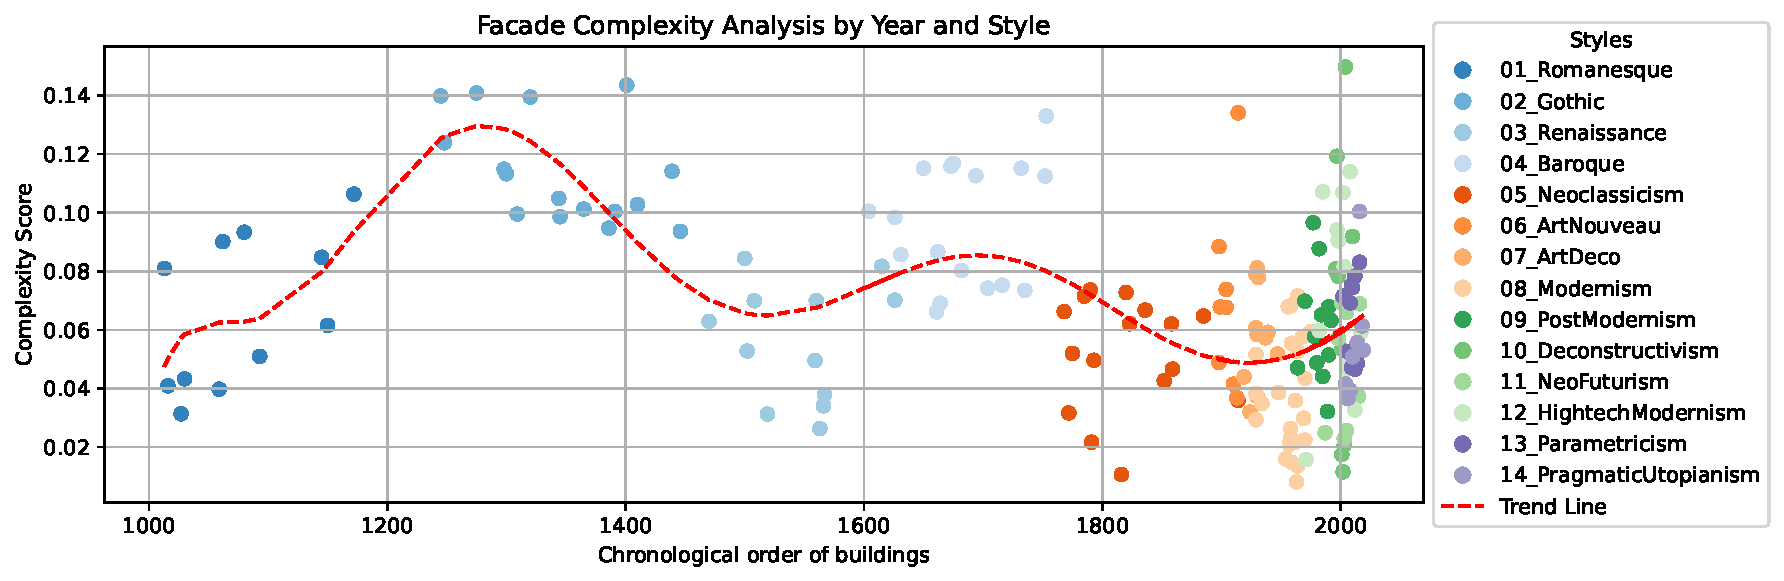
\includegraphics[width= \linewidth]{Graphs/complexitygraph}
          \caption{Scatter graph showcasing quantitative image complexity analysis scores for building images categorized by historical timeline and architectural style, with an overlaid trendline highlighting the evolving trend towards increased complexity.}
          \label{fig:HistoricalComplexityGraph}
     \end{figure*}










We have previously discussed the argument that the architectural evolution, throughout history, has been characterized by a continual interplay between simplicity and complexity.
This notion has been substantiated by our exploration of the theoretical definitions and varied approaches to facades and ornamentation within the context of prominent architectural styles and the perspectives of their eminent architects.

Our literature review has consistently pointed towards a prevailing trend in contemporary architecture, suggesting a resurgence of complexity in architectural design.
However, to ensure our findings are not purely subjective or biased towards this conclusion, we have conducted a quantitative analysis using the Computational Image Complexity Analysis (CICA) system.
This rigorous analysis method utilizes input images of the most iconic and representative buildings from various epochs and styles.

The results are visually depicted in Figure\ref{fig:HistoricalComplexityGraph}, where a discernible upward trendline towards complexity emerges, particularly noticeable since the late 20th century.

%% Figure of Complexity graph
     \begin{figure*}[!htb]
          \centering
          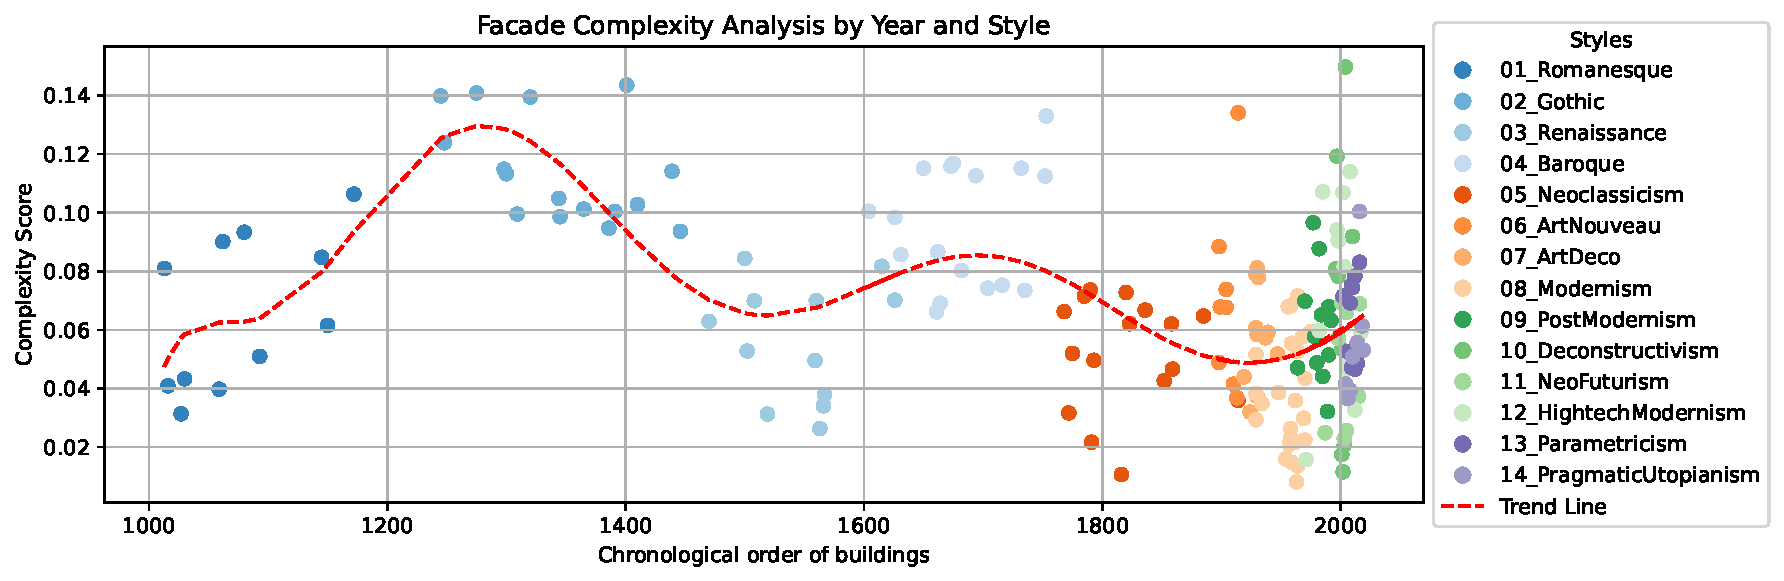
\includegraphics[width= \linewidth]{Graphs/complexitygraph}
          \caption{Scatter graph showcasing quantitative image complexity analysis scores for building images categorized by historical timeline and architectural style, with an overlaid trendline highlighting the evolving trend towards increased complexity.}
          \label{fig:HistoricalComplexityGraph}
     \end{figure*}










We have previously discussed the argument that the architectural evolution, throughout history, has been characterized by a continual interplay between simplicity and complexity.
This notion has been substantiated by our exploration of the theoretical definitions and varied approaches to facades and ornamentation within the context of prominent architectural styles and the perspectives of their eminent architects.

Our literature review has consistently pointed towards a prevailing trend in contemporary architecture, suggesting a resurgence of complexity in architectural design.
However, to ensure our findings are not purely subjective or biased towards this conclusion, we have conducted a quantitative analysis using the Computational Image Complexity Analysis (CICA) system.
This rigorous analysis method utilizes input images of the most iconic and representative buildings from various epochs and styles.

The results are visually depicted in Figure\ref{fig:HistoricalComplexityGraph}, where a discernible upward trendline towards complexity emerges, particularly noticeable since the late 20th century.

%% Figure of Complexity graph
     \begin{figure*}[!htb]
          \centering
          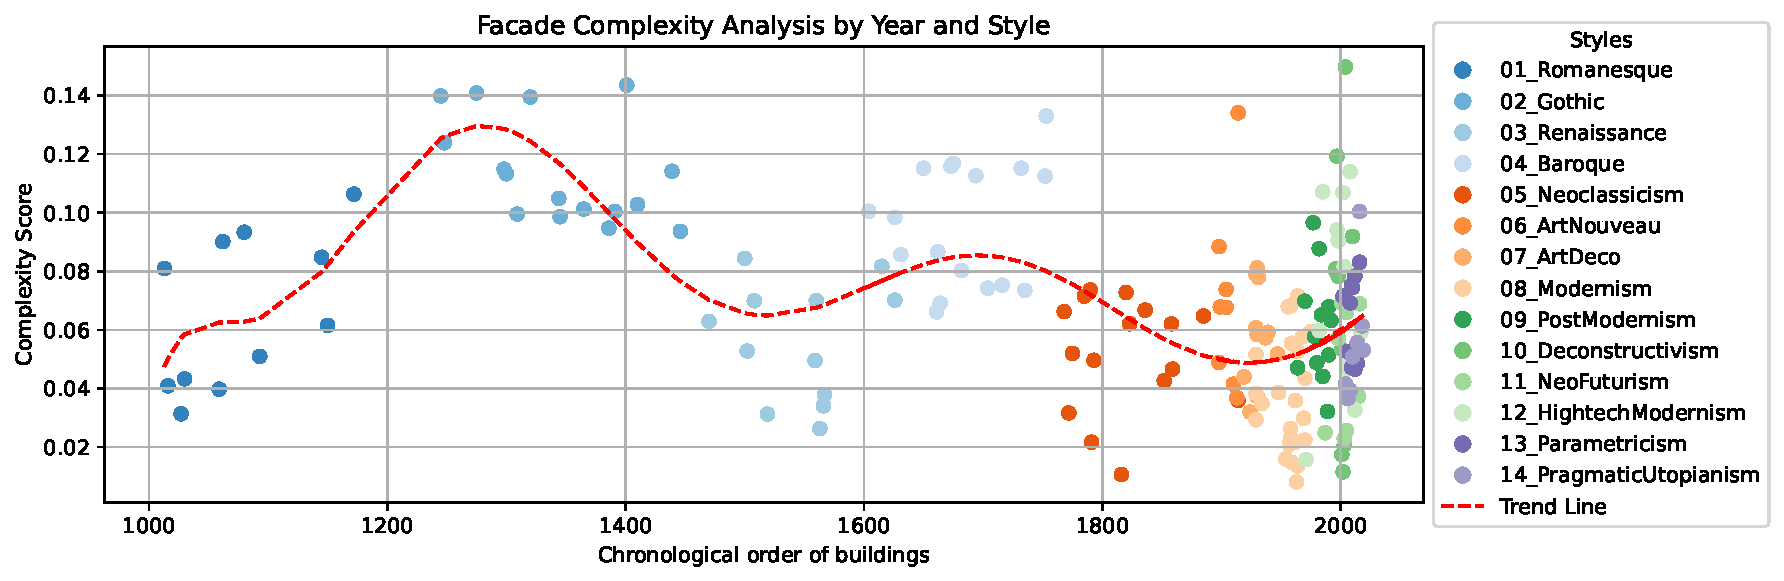
\includegraphics[width= \linewidth]{Graphs/complexitygraph}
          \caption{Scatter graph showcasing quantitative image complexity analysis scores for building images categorized by historical timeline and architectural style, with an overlaid trendline highlighting the evolving trend towards increased complexity.}
          \label{fig:HistoricalComplexityGraph}
     \end{figure*}











We have previously discussed the argument that the architectural evolution, throughout history, has been characterized by a continual interplay between simplicity and complexity.
This notion has been substantiated by our exploration of the theoretical definitions and varied approaches to facades and ornamentation within the context of prominent architectural styles and the perspectives of their eminent architects.

Our literature review has consistently pointed towards a prevailing trend in contemporary architecture, suggesting a resurgence of complexity in architectural design.
However, to ensure our findings are not purely subjective or biased towards this conclusion, we have conducted a quantitative analysis using the Computational Image Complexity Analysis (CICA) system.
This rigorous analysis method utilizes input images of the most iconic and representative buildings from various epochs and styles.

The results are visually depicted in Figure\ref{fig:complexitygraph}, where a discernible upward trendline towards complexity emerges, particularly noticeable since the late 20th century.

%% Figure of Complexity graph
     \begin{figure*}[!htb]
          \centering
          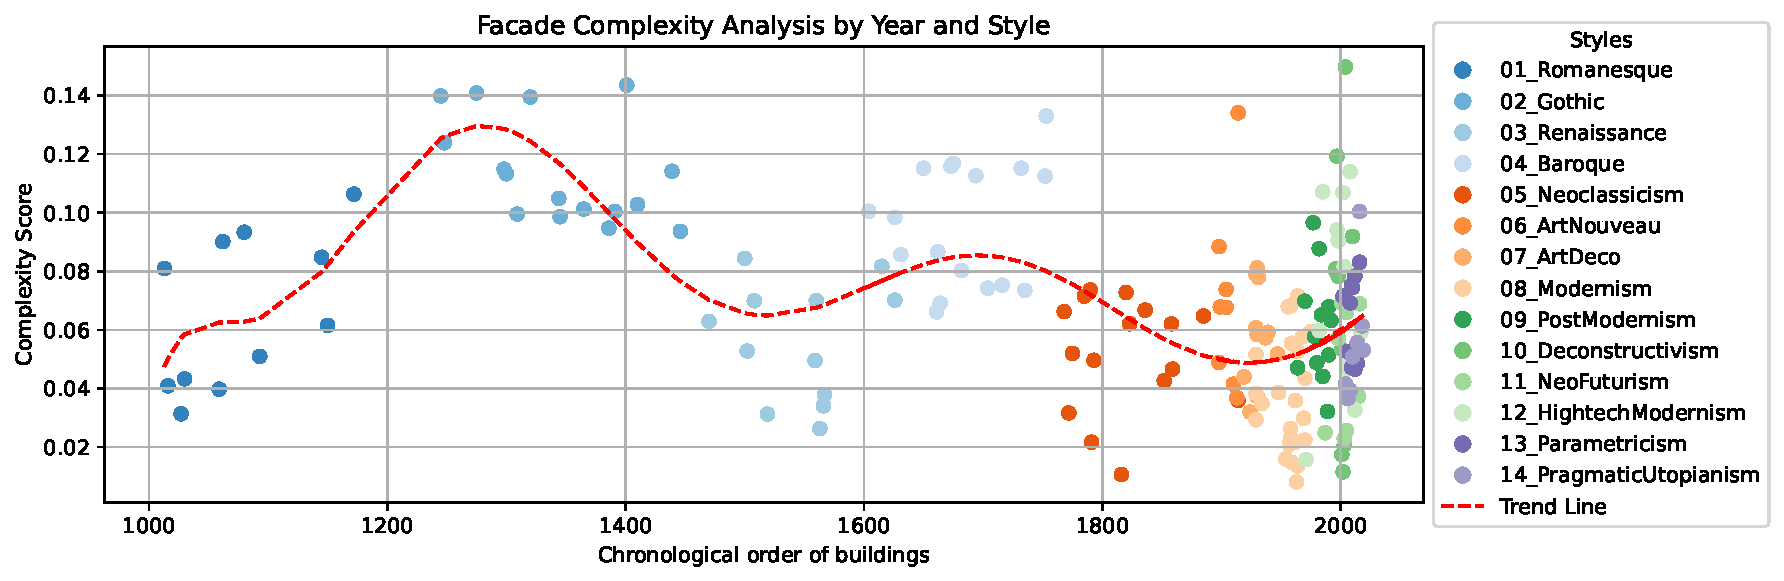
\includegraphics[width= \linewidth]{Graphs/complexitygraph}
          \caption{Scatter graph showcasing quantitative image complexity analysis scores for building images categorized by historical timeline and architectural style, with an overlaid trendline highlighting the evolving trend towards increased complexity.}
          \label{fig:complexitygraph}
     \end{figure*}








